\documentclass[fontsize=12pt,paper=a4,twoside]{scrartcl}

\newcommand{\grad}{\ensuremath{^{\circ}} }
\renewcommand{\strut}{\vrule width 0pt height5mm depth2mm}

\usepackage[utf8]{inputenc}
\usepackage[final]{pdfpages}
% obere Seitenränder gestalten können
\usepackage{fancyhdr}
\usepackage{moreverb}
% Graphiken als jpg, png etc. einbinden können
\usepackage{graphicx}
\usepackage{stmaryrd}
% Floats Objekte mit [H] festsetzen
\usepackage{float}
% setzt URL's schön mit \url{http://bla.laber.com/~mypage}
\usepackage{url}
% Externe PDF's einbinden können
\usepackage{pdflscape}
% Verweise innerhalb des Dokuments schick mit " ... auf Seite ... "
% automatisch versehen. Dazu \vref{labelname} benutzen
\usepackage[ngerman]{varioref}
\usepackage[ngerman]{babel}
\usepackage{ngerman}
% Bibliographie
\usepackage{bibgerm}
% Tabellen
\usepackage{tabularx}
\usepackage{supertabular}
\usepackage[colorlinks=true, pdfstartview=FitV, linkcolor=blue,
            citecolor=blue, urlcolor=blue, hyperfigures=true,
            pdftex=true]{hyperref}
\usepackage{bookmark}

\hyphenation{Arbeits-paket}

\newboolean{langversion} %Deklaration
\setboolean{langversion}{true} %Zuweisung ist 'false' für Blockkurs
\newcommand{\highlight}[1]{\textcolor{blue}{\textbf{#1}}}
\newcommand{\nurlangversion}[0]{%
\ifthenelse{\boolean{langversion}}{\highlight{Muss in SWP-2 ausgefüllt werden}}{\highlight{Entfällt in SWP-1}}}


\newcommand{\swp}[0]{\ifthenelse{\boolean{langversion}}%
{Software--Projekt 2}{Software--Projekt 1}}
\newcommand{\jahr}[0]{2014}
\newcommand{\semester}[0]{\ifthenelse{\boolean{langversion}}{WiSe}{SoSe}}

% erstes Argument: SWP-2, zweites SWP-1
\newcommand{\variante}[2]{\ifthenelse{\boolean{langversion}}{#1}{#2}}

% Damit Latex nicht zu lange Zeilen produziert:
\sloppy
%Uneinheitlicher unterer Seitenrand:
%\raggedbottom

% Kein Erstzeileneinzug beim Absatzanfang
% Sieht aber nur gut aus, wenn man zwischen Absätzen viel Platz einbaut
\setlength{\parindent}{0ex}

% Abstand zwischen zwei Absätzen
\setlength{\parskip}{1ex}

% Seitenränder für Korrekturen verändern
\addtolength{\evensidemargin}{-1cm}
\addtolength{\oddsidemargin}{1cm}

\bibliographystyle{gerapali}

% Lustige Header auf den Seiten
  \pagestyle{fancy}
  \setlength{\headheight}{70.55003pt}
  \fancyhead{}
  \fancyhead[LO,RE]{\swp\\ \semester \jahr
  \\Architekturbeschreibung}
  \fancyhead[LE,RO]{Seite \thepage\\\slshape \leftmark\\\slshape \rightmark}

%Etwas größere Zeilenabstände in Tabellen
\renewcommand{\arraystretch}{1.2}

%
% Und jetzt geht das Dokument los....
%

\begin{document}

% Lustige Header nur auf dieser Seite
  \thispagestyle{fancy}
  \fancyhead[LO,RE]{ }
  \fancyhead[LE,RO]{Universität Bremen\\FB 3 -- Informatik\\
  Prof. Dr. Rainer Koschke \\TutorIn: Karsten Hölscher}
  \fancyfoot[C]{}

% Start Titelseite
  \vspace{3cm}

  \begin{minipage}[H]{\textwidth}
  \begin{center}
  \bf
  \Large
  Software--Projekt 2 2014\\
  \smallskip
  \small
  VAK 03-BA-901.02\\
  \vspace{3cm}
  \end{center}
  \end{minipage}
  \begin{minipage}[H]{\textwidth}
  \begin{center}
  \vspace{1cm}
  \bf
  \Large Architekturbeschreibung\\
  \vspace{3ex}
   	  \begin{figure}[H]
      \centering
      
\includegraphics[width=0.25\textwidth]{../WOYM.png}
      \end{figure}
  \vfill
  \end{center}
  \end{minipage}
  \vfill
  \begin{minipage}[H]{\textwidth}
  \begin{center}
  \sf
  \begin{tabular}{l}
  Tim Hansen \\
  Adrian Lück \\
  Jurij Schmidt\\
  \end{tabular}
  \\ ~
  \vspace{2cm}
  \\
  \it Version 1.2\\ ~
  \end{center}
  \end{minipage}

% Ende Titelseite

% Start Leerseite

\newpage

  \thispagestyle{fancy}
  \fancyhead{}
  \fancyhead[LO,RE]{\swp{} \\  \semester{} \jahr{}
  \\Architekturbeschreibung}
  \fancyhead[LE,RO]{Seite \thepage\\\slshape \leftmark\\~}
  \fancyfoot{}
  \renewcommand{\headrulewidth}{0.4pt}
  \tableofcontents

\newpage

  \fancyhead[LE,RO]{Seite \thepage\\\slshape \leftmark\\\slshape \rightmark}


%%%%%%%%%%%%%%%%%%%%%%%%%%%%%%%%%%%%%%%%%%%%%%%%%%%%%%%%%%%%%%%%%%%%%%%%
\section*{Version und Änderungsgeschichte}

\begin{tabular}{ccl}
Version & Datum & Änderungen \\
\hline
1.0 & 29.10.2014 & Dokumentvorlage als initiale Fassung kopiert  \\
1.1 & 22.11.2014 & Erste vollständige Fassung der konzeptionellen und Datensicht\\
1.2 & 17.01.2015 & Paketdiagramm hinzugefügt. Datenmodell aktualisiert. \\
\end{tabular}


%%%%%%%%%%%%%%%%%%%%%%%%%%%%%%%%%%%%%%%%%%%%%%%%%%%%%%%%%%%%%%%%%%%%%%%%
\section{Einführung}

\subsection{Zweck}
  
Die Architekturbeschreibung soll es anderen Entwicklern ermöglichen, den Aufbau der Software und Intentionen hinter bestimmten Design-Entscheidungen zu verstehen. Dadurch sollen Fremdentwickler in die Lage versetzt werden, die Software zu überarbeiten und Bugs zu beheben.

\subsection{Status}
Dieses Dokument gibt die Software-Architektur des finalen Produktes wieder.


  
\subsection{Definitionen, Akronyme und Abkürzungen}


\subsection{Referenzen}
Die folgenden Kapitel stützen sich im Wesentlichen auf die Vorlesungsfolien "`Software-Architektur 1"' der Veranstaltung "`Software-Projekt 1"' im Sommersemester 2014 an der Universität Bremen von Prof. Dr. Rainer Koschke.


\subsection{Übersicht über das Dokument}
\nurlangversion


\section{Globale Analyse}
\label{sec:globale_analyse}

\subsection{Einflussfaktoren}
\label{sec:einflussfaktoren}
{\it Hier sind Einflussfaktoren gefragt, die sich auf die Architektur
  beziehen. Es sind ausschließlich architekturrelevante
  Einflussfaktoren, und nicht z.B.\ solche, die lediglich einen
  Einfluss auf das Projektmanagement haben. Fragt Euch also bei jedem
  Faktor: Beeinflusst er wirklich die Architektur? Macht einen
  einfachen Test: Wie würde die Architektur aussehen, wenn ihr den
  Einflussfaktor E berücksichtigt? Wie würde sie aussehen, wenn Ihr E nicht
  berücksichtigt? Kommt in beiden Fällen dieselbe Architektur heraus,
  dann kann der Einflussfaktor nicht architekturrelevant sein.

  Es geht hier um Einflussfaktoren, die
  \begin{enumerate}
  \item sich über die Zeit ändern,
  \item viele Komponenten betreffen,
  \item schwer zu erfüllen sind oder
  \item mit denen man wenig Erfahrung hat.
  \end{enumerate}
  Die Flexibilität und Veränderlichkeit müssen ebenfalls charakterisiert werden. 
  \begin{enumerate}
  \item Flexibilität: Könnt Ihr den Faktor zum jetzigen Zeitpunkt beeinflussen?
  \item Veränderlichkeit: ändert der Faktor sich später durch äußere Einflüsse?
\end{enumerate}

  Unter Auswirkungen sollte dann beschrieben werden, {\em wie} der
  Faktor {\em was} beeinflusst. Das können sein:
  \begin{itemize}
  \item andere Faktoren
  \item Komponenten
  \item Operationsmodi
  \item Designentscheidungen (Strategien)
  \end{itemize}

  Verwendet eine eindeutige Nummerierung der Faktoren, um sie auf den
  Problemkarten einfach referenzieren zu können.  }\\

\subsubsection{Organisatorische Faktoren}
\renewcommand{\arraystretch}{1.4}
\begin{tabularx}{\textwidth}{|X|X|X|}
\hline
\textbf{Faktor} & \textbf{Flexibilität und Veränderlichkeit} & \textbf{Auswirkungen}\\\hline
\hline
\multicolumn{3}{|l|}{\textbf{O1: Management}}\\\hline
\multicolumn{3}{|l|}{O1.1: Zeitplan vs. Funktionsumfang}\\\hline
Der Zeitplan ist in jedem Fall einzuhalten. Ggf. muss dafür in Kauf genommen werden, dass gewisse Funktionen fehlen. & Dieser Faktor ist nicht flexibel oder veränderlich. & Nicht alle geplanten Funktionen können implementiert werden. Zunächst Beschränkung auf die Funktionen, die notwendig sind, um die Mindestanforderungen zu erfüllen.\\\hline

\multicolumn{3}{|l|}{\textbf{O2: Personal: Fähigkeiten, Interessen, Stärken, Schwächen}}\\\hline
\multicolumn{3}{|l|}{O2.1: Erstes größeres, selbständig auszuführendes Projekt}\\\hline
Für alle beteiligten Entwickler handelt es sich um das erste größere selbstständig auszuführende Projekt. & Dieser Faktor ist nicht flexibel oder veränderlich. & %TODO 
\\\hline

\multicolumn{3}{|l|}{\textbf{O3: Prozesse und Werkzeuge für die Entwicklungsschritte}}\\\hline

\multicolumn{3}{|l|}{\textbf{O4: Entwicklungszeitplan}}\\\hline
\multicolumn{3}{|l|}{O4.1: Auslieferung der Produktfunktionen}\\\hline
Es werden die absolut notwendigen Produktfunktionen (Mindestanforderungen) priorisiert. & Die Mindestanforderungen und damit die Prioritätensetzung können sich im Zeitverlauf verändern (inbes. abhängig von O5.1). & Kann O1.1 beeinflussen.\\\hline

\multicolumn{3}{|l|}{\textbf{O5: Entwicklungsbudget}}\\\hline
\multicolumn{3}{|l|}{O5.1: Anzahl der Entwickler}\\\hline
Es sind maximal sechs Entwickler am Projekt beteiligt. & Es können keine weitere Entwickler hinzugezogen werden. Teilnehmende Entwickler können temporär oder komplett ausfallen. & Ein temporärer Ausfall kann Faktor 01.1 leicht beeinflussen. Bei komplettem Ausfall eines Entwicklers werden die Mindestanforderungen verändert und damit O4.1 und O1.1 beeinflusst.\\\hline
\end{tabularx}\\
\clearpage

\subsubsection{Technische Faktoren}

\begin{tabularx}{\textwidth}{|X|X|X|}
\hline
\textbf{Faktor} & \textbf{Flexibilität und Veränderlichkeit} & \textbf{Auswirkungen}\\\hline
\hline
\multicolumn{3}{|l|}{\textbf{T1: Hardware}}\\\hline
\multicolumn{3}{|l|}{T1.1: Hardwarelandschaft des Kunden ist zu berücksichtigen}\\\hline
Die Software muss auf einem Rechner mit 4 GB RAM, 70 GB Festplattenspeicher, einer Dual-Core-CPU mit 2,9 GHz Takt lauffähig sein und auf einem Monitor mit einer Auflösung von 1280 x 1024 korrekt dargestellt werden. & Dieser Faktor ist nicht flexibel. In Zukunft könnte sich die Hardwarelandschaft des Kunden jedoch verändern, wobei davon auszugehen ist, dass höchstens ein Up- und kein Downgrade stattfindet. & %TODO
 \\\hline

\multicolumn{3}{|l|}{\textbf{T2: Software}}\\\hline
\multicolumn{3}{|l|}{T2.1: Betriebssystem}\\\hline
Die Software soll auf allen gängigen Betriebssystemen (Microsoft Windows, Linux, Mac-OS) lauffähig sein. & Dieser Faktor ist nicht flexibel, aber ggf. veränderlich, da neue Betriebssystem erscheinen können. & Bei der Entwicklung muss darauf geachtet werden, betriebssystemunabhängige Komponenten zu verwenden.\\\hline
\multicolumn{3}{|l|}{T2.2: Verwendung von JavaServer Faces bzw. Primefaces}\\\hline
Für die grafische Darstellung der Software wird JavaServer Faces bzw. Primefaces verwendet. & Dieser Faktor könnte zu Beginn noch verändert werden, eine Veränderung zu einem späteren Zeitpunkt wäre eher unwahrscheinlich. & Nimmt starken Einfluss auf die Implementierung der View- und der Controller-Komponente. Alle Datenklassen benötigen außerdem Getter- und Setter-Methoden für alle ihre Attribute. \\\hline
\end{tabularx} \clearpage

\begin{tabularx}{\textwidth}{|X|X|X|}
\hline
\textbf{Faktor} & \textbf{Flexibilität und Veränderlichkeit} & \textbf{Auswirkungen}\\\hline
\hline
\multicolumn{3}{|l|}{T2.3: Verwendung der JPA-Implementierung Eclipselink}\\\hline
Für die Anbindung an das relationale Datenbanksystem wird das JPA-Framework Eclipselink verwendet. & Dieser Faktor ist flexibel, es könnte grundsätzlich auch jedes andere JPA-Framework gewählt werden bzw. auch gar keines solcher Frameworks. Theoretisch ist der Faktor auch veränderlich. Wenn etwa Probleme mit dem Framework auftreten könnte in Betracht gezogen werden, es durch ein anderes auszutauschen. & Dieser Faktor beeinflusst vor allem die Implementierung der Persistenz-Komponente. \\\hline
\multicolumn{3}{|p{\dimexpr\textwidth-2\tabcolsep\relax}|}{T2.4: Verwendung des Command-Entwurfmusters in Kombination mit dem Composite- und Memento-Entwurfmuster}\\\hline
Für die geeignete Erfüllung von Faktor P1.1 soll das Command-Entwurfsmuster in Kombination mit dem Composite- und Memento-Entwurfsmuster implementiert werden. Das Composite-Entwurfsmuster würde dann die Erstellung von Macro-Commands erlauben. Das Memento-Entwurfsmuster erlaubt die gekapselte Datenspeicherung für Update-Commands. & Dieser Faktor ist flexibel und gemäß P1.1 veränderlich. & Beeinflusst die Implementierung der Model-Komponente deutlich. Da die gesamte Logik für das Speichern, Aktualisieren und Löschen von Objekten auf Commands aufgebaut sein muss. Zudem müssen alle notwendigen Klassen eine eigene Memento-Klasse besitzen. \\\hline
\end{tabularx}

\begin{tabularx}{\textwidth}{|X|X|X|}
\hline
\textbf{Faktor} & \textbf{Flexibilität und Veränderlichkeit} & \textbf{Auswirkungen}\\\hline
\hline
\multicolumn{3}{|l|}{T2.5: Verwendung des Factory-Patterns für Delete-Commands}\\\hline
Geht aus dem Faktor T2.4 hervor. Da beim Löschen von Objekten einige Abhängigkeiten zu berücksichtigen sind, damit es in der Datenbank nicht zu Fremdschlüssel-Verletzungen kommt, bietet sich die Implementierung einer Klasse, die Macro-Delete-Commands unter Berücksichtigung der Abhängigkeiten erzeugt, nach dem Factory-Pattern an.& Dieser Faktor ist flexibel und gemäß 2.4 veränderlich. & Beeinflusst die Implementierung der Model-Komponente. \\\hline
\multicolumn{3}{|l|}{\textbf{T3: Architekturtechnologie}}\\\hline

\multicolumn{3}{|l|}{\textbf{T4: Standards}}\\\hline
\multicolumn{3}{|l|}{T4.1: Leichtgewichtiges eingebettetes relationales Datenbanksystem}\\\hline
Die Verwendung einer leichtgewichtigen, eingebetteten relationalen Datenbank ist vorgeschrieben. & Dieser Faktor ist nicht flexibel oder veränderlich. & \\\hline
\end{tabularx}

\clearpage

\subsubsection{Produktfaktoren}
\begin{tabularx}{\textwidth}{|X|X|X|}
\hline
\textbf{Faktor} & \textbf{Flexibilität und Veränderlichkeit} & \textbf{Auswirkungen}\\\hline
\hline
\multicolumn{3}{|l|}{\textbf{P1: Produktfunktionen}}\\\hline
\multicolumn{3}{|l|}{P1.1: Mehrstufiges Rückgängigmachen von Aktionen}\\\hline
Um die Lernförderlichkeit zu unterstützen, soll es den Benutzern möglich sein, Aktionen mehrstufig rückgängig zu machen. & Dieser Faktor ist nicht flexibel, kann im Zuge von O4.1 jedoch ggf. wegfallen. & Bei der Planung und Implementierung der Geschäftslogik muss darauf geachtet werden, diesen Faktor geeignet zu berücksichtigen. Aus diesem Einflussfaktor geht T2.3 hervor.
\\\hline
\multicolumn{3}{|l|}{P1.2: Systemeinstellungen}\\\hline
Die Software soll verschieden Systemeinstellungen bieten, die etwa erlauben, zu verplanende Wochentage, Start- und Ende eines Wochentages, Backup-Einstellungen usw. festzulegen. & Dieser Faktor ist nicht flexibel, kann im Zuge von O4.1 aber ggf. wegfallen. & Es muss eine Möglichkeit geben, solcherlei Einstellungen zu verändern und sie über einen Systemstart hinaus zu speichern.\\\hline
\multicolumn{3}{|l|}{\textbf{P2: Benutzerschnittstelle}}\\\hline

\multicolumn{3}{|l|}{\textbf{P3: Performanz}}\\\hline

\multicolumn{3}{|l|}{\textbf{P4: Verlässlichkeit}}\\\hline

\multicolumn{3}{|l|}{\textbf{P5: Fehlererkennung, -bericht, -behandlung}}\\\hline

\multicolumn{3}{|l|}{\textbf{P6: Service}}\\\hline
\end{tabularx}\\


\subsection{Probleme und Strategien}
\label{sec:strategien}

{\it Aus einer Menge von Faktoren ergeben sich Probleme, die nun in
  Form von Problemkarten beschrieben werden. Diese resultieren
  z.B. aus
  \begin{itemize}
  \item Grenzen oder Einschränkungen durch Faktoren
  \item der Notwendigkeit, die Auswirkungen eines Faktors zu begrenzen
  \item der Schwierigkeit, einen Produktfaktor zu erfüllen, oder
  \item der Notwendigkeit einer allgemeinen Lösung zu globalen
    Anforderungen.
  \end{itemize}
  Dazu entwickelt Ihr Strategien, um mit den identifizierten Problemen
  umzugehen.

  Achtet auch hier darauf, dass die Probleme und Strategien wirklich
  die Architektur betreffen und nicht etwa das Projektmanagement. Die
  Strategien stellen im Prinzip die Designentscheidungen dar. Sie
  sollten also die Erklärung für den konkreten Aufbau der
  verschiedenen Sichten liefern.}


\textit{Beschreibt möglichst mehrere Alternativen und gebt
  an, für welche Ihr Euch letztlich aus welchem Grunde entschieden
  habt. Natürlich müssen die genannten Strategien in den folgenden
  Sichten auch tatsächlich umgesetzt werden!}

\textit{Ein sehr häufiger Fehler ist es, dass SWP-Gruppen
  arbeitsteilig vorgehen: die eine Gruppe schreibt das Kapitel zur
  Analyse von Faktoren und zu den Strategien, die andere Gruppe
  beschreibt die diversen Sichten, ohne dass diese beiden Gruppen sich
  abstimmen. Natürlich besteht aber ein Zusammenhang zwischen den
  Faktoren, Strategien und Sichten. Dieser muss erkennbar sein, indem
  sich die verschiedenen Kapitel eindeutig aufeinander beziehen.}

\section{Konzeptionelle Sicht}
\label{sec:konzeptionell}

%TODO: Diagramm und Beschreibung überarbeiten

Der Client besteht aus der GUI-, Model- und Persistence-Komponente. Die GUI-Komponente ist wiederum unterteilt in View und Controller. Die View-Komponente stellt Daten (in Form von Eingaben des Nutzers) für den Controller bereit. Der Controller hat die Kontrolle über die View-Komponente. Der Controller gibt die von der View-Komponente erhaltenen Daten nach ggf. ersten Validierungen in Form eines Transferobjektes an die Model-Komponenten weiter. Diese implementiert die Logik des Systems. Die Model-Komponente verarbeitet also die erhaltenen Daten, führt ggf. Berechnungen aus und gibt dem Controller in der Regel ein Status-Objekt zurück, welches den Erfolg oder Misserfolg (inkl. Gründen) einer Datenverarbeitung angibt. \\
Auf unterster Ebene befindet sich schließlich die Persistence-Komponente. Diese hat die Kontrolle über die Datenbank und führt dementsprechend die Datenbankanfragen aus. Die Persistence-Komponente wird nur von der Model-Komponente aufgerufen, nicht von der GUI. Die Architektur folgt also dem Schichtenmodell.

\section{Modulsicht}
\label{sec:modulsicht}

{\it
Diese Sicht beschreibt den statischen Aufbau des Systems mit Hilfe von
Modulen, Subsystemen, Schichten und Schnittstellen. 
Diese Sicht ist hierarchisch, d.h. Module werden in Teilmodule
zerlegt. Die Zerlegung endet bei Modulen, die ein klar umrissenes
Arbeitspaket für eine Person darstellen und in einer Kalenderwoche
implementiert werden können. Die Modulbeschreibung der Blätter dieser
Hierarchie muss genau genug und ausreichend sein, um das Modul 
implementieren zu können.

Die Modulsicht wird durch {UML}-Paket- und Klassendiagramme visualisiert.

Die Module werden durch ihre Schnittstellen beschrieben. 
Die Schnittstelle eines Moduls $M$ ist die Menge aller Annahmen, die
andere Module über $M$ machen dürfen, bzw.\ jene Annahmen, die $M$
über seine verwendeten Module macht (bzw. seine Umgebung, wozu auch
Speicher, Laufzeit etc.\ gehören).
Konkrete Implementierungen dieser Schnittstellen sind das Geheimnis des Moduls
und können vom Programmierer festgelegt werden. Sie sollen hier
dementsprechend nicht beschrieben werden. 

Die Diagramme der Modulsicht sollten die zur Schnittstelle gehörenden Methoden
enthalten. Die Beschreibung der einzelnen Methoden (im Sinne der Schnittstellenbeschreibung)
geschieht allerdings per Javadoc im zugehörigen Quelltext. Das bedeutet, dass Ihr
für alle Eure Module Klassen, Interfaces und Pakete erstellt und sie mit den Methoden der
Schnittstellen verseht. Natürlich noch ohne Methodenrümpfe bzw.\ mit minimalen Rümpfen.
Dieses Vorgehen vereinfacht den Schnittstellenentwurf und stellt Konsistenz sicher.

Jeder Schnittstelle liegt ein
Protokoll zugrunde. Das Protokoll beschreibt die Vor- und
Nachbedingungen der Schnittstellenelemente. Dazu gehören die erlaubten
Reihenfolgen, in denen Methoden der Schnittstelle aufgerufen werden
dürfen, sowie Annahmen über Eingabeparameter und Zusicherungen über
Ausgabeparameter. Das Protokoll von Modulen wird in der Modulsicht beschrieben.
Dort, wo es sinnvoll ist, sollte es mit Hilfe von Zustands- oder
Sequenzdiagrammen spezifiziert werden. Diese sind dann einzusetzen, wenn der
Text allein kein ausreichendes Verständnis vermittelt (insbesondere
bei komplexen oder nicht offensichtlichen Zusammenhängen).

Der Bezug zur konzeptionellen Sicht muss klar ersichtlich sein. Im
Zweifel sollte er explizit erklärt werden. Auch für diese Sicht muss
die Entstehung anhand der Strategien erläutert werden.
}

\subsection{Paketdiagramm}
Die Software ist aufgeteilt in fünf große Pakete, die jeweils noch Unterpakte besitzen. In dem nachfolgend aufgeführten Paketdiagramm sind nur die Abhängigkeiten zwischen den großen Pakten aufgeführt, um es übersichtlicher zu halten. Im Paket \textit{org.woym.persistence} befinden sich alle Klassen die in irgendeiner Weise eine Verbindung mit der Datenbank unterhalten, im Unterpaket \textit{org.woym.persistence.spec} befinden sich die zugehörigen Interfaces (s. Kapitel \ref{sec:persistence}).\\ Im Paket \textit{org.woym.common} bzw. in den jeweiligen Unterpaketen befinden sich Klassen, welche von Klassen aus fast allen anderen Paketen verwendet werden.\\
Das Paket \textit{org.woym.controller} enthält alle Controller, welche die Eingaben von der GUI verarbeiten. Im Paket \textit{org.woym.ui} befinden sich JSF-Validatoren und Converter. \\ 
Im Paket \textit{org.woym.logic} befinden sich alle Klassen, die die Geschäftslogik implementieren (s. Kapitel \ref{sec:logic}).

\begin{figure}[H]
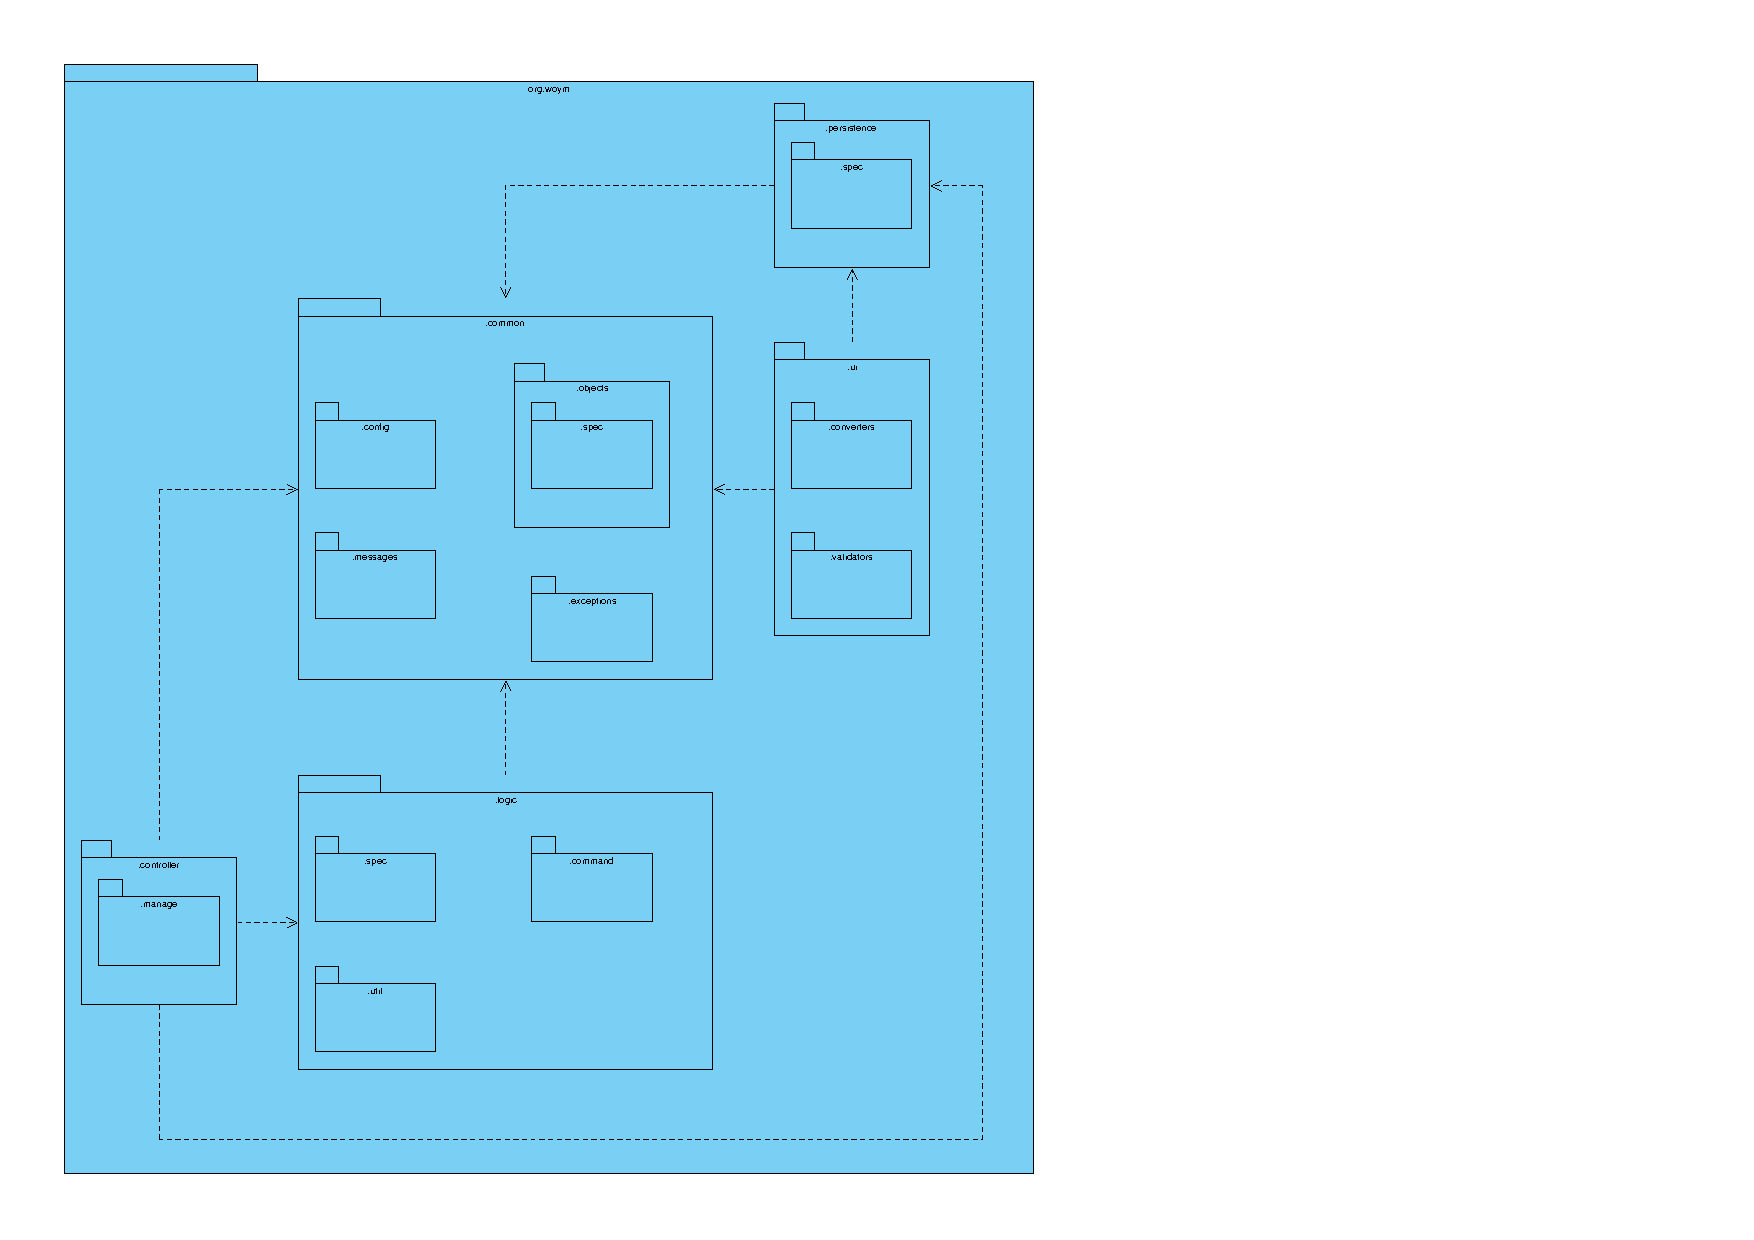
\includegraphics[width=\textwidth]{packages.pdf}
\end{figure}


\subsection{Common}
Im Paket \textit{org.woym.common} befinden sich -- wie vorher bereits angemerkt -- Klassen, welche von Klassen aus fast allen anderen Paketen verwendet werden.\\
Das Paket \textit{org.woym.common.config} beinhaltet das \texttt{DefaultConfigEnum}, welches alle Einstellungsoptionen der Software mit ihren Standardwerten enthält. Die Klasse \texttt{Config} erzeugt eine Properties-Datei und gewährt anderen Klassen Zugriff auf dort eingetragene Werte. Bevor die anderen Methoden der Klasse aufgerufen werden können, muss mindestens einmal die Methode \textit{init()} aufgerufen werden. %TODO: Ggf. etwas erweitern/umschreiben 
\\
Die Klasse \texttt{ConfigServletListener} implementiert das Java-Interface \texttt{ServletContextListener} und sorgt dafür, dass mit dem Start des Servlet-Containers einmal die \textit{init()}-Methode von \texttt{Config} aufgerufen wird.\\

Das Paket \textit{org.woym.common.messages} beinhaltet vier Enums mit Statusnachrichten. Die Klasse \texttt{MessageHelper} stellt Methoden bereit, welche für die Übergabe einer entsprechenden Nachricht und ggf. zusätzlichen Parametern eine \texttt{FaceMessage} zurückgibt. Die Methoden können in beliebiger Reihenfolge aufgerufen werden.\\

Das Paket \textit{org.woym.common.exceptions} enthält lediglich die selbst angelegten Exceptions. \\

Das Paket \textit{org.woym.common.objects} ist hier nicht vollständig dargestellt (s. Kapitel \ref{subsubsec:Objects}), da dies zu unübersichtlich wäre, stattdessen ist nur das Unterpaket \textit{org.woym.common.objects.spec} dargestellt. Dieses enthält drei Interfaces. \texttt{IMemento} dient lediglich der Vereinheitlichung aller einzelnen Memento-Klassen unter einem gemeinsamen Interface. Da die Memento-Klassen nach außen hin vollständig opak sind und keinerlei Methoden bereitstellen, können sie unter diesem Interface vereinheitlicht werden. Das Interface \texttt{IActivityObject} dient der Vereinheitlichung von Klassen, deren Objekte Teil der Klasse \texttt{Activity} sein können. \\
Das Interface \texttt{IMementoObject} stellt Methoden für alle Klassen bereit, welche eine eigene Memento-Klasse definieren.


\begin{figure}[H]
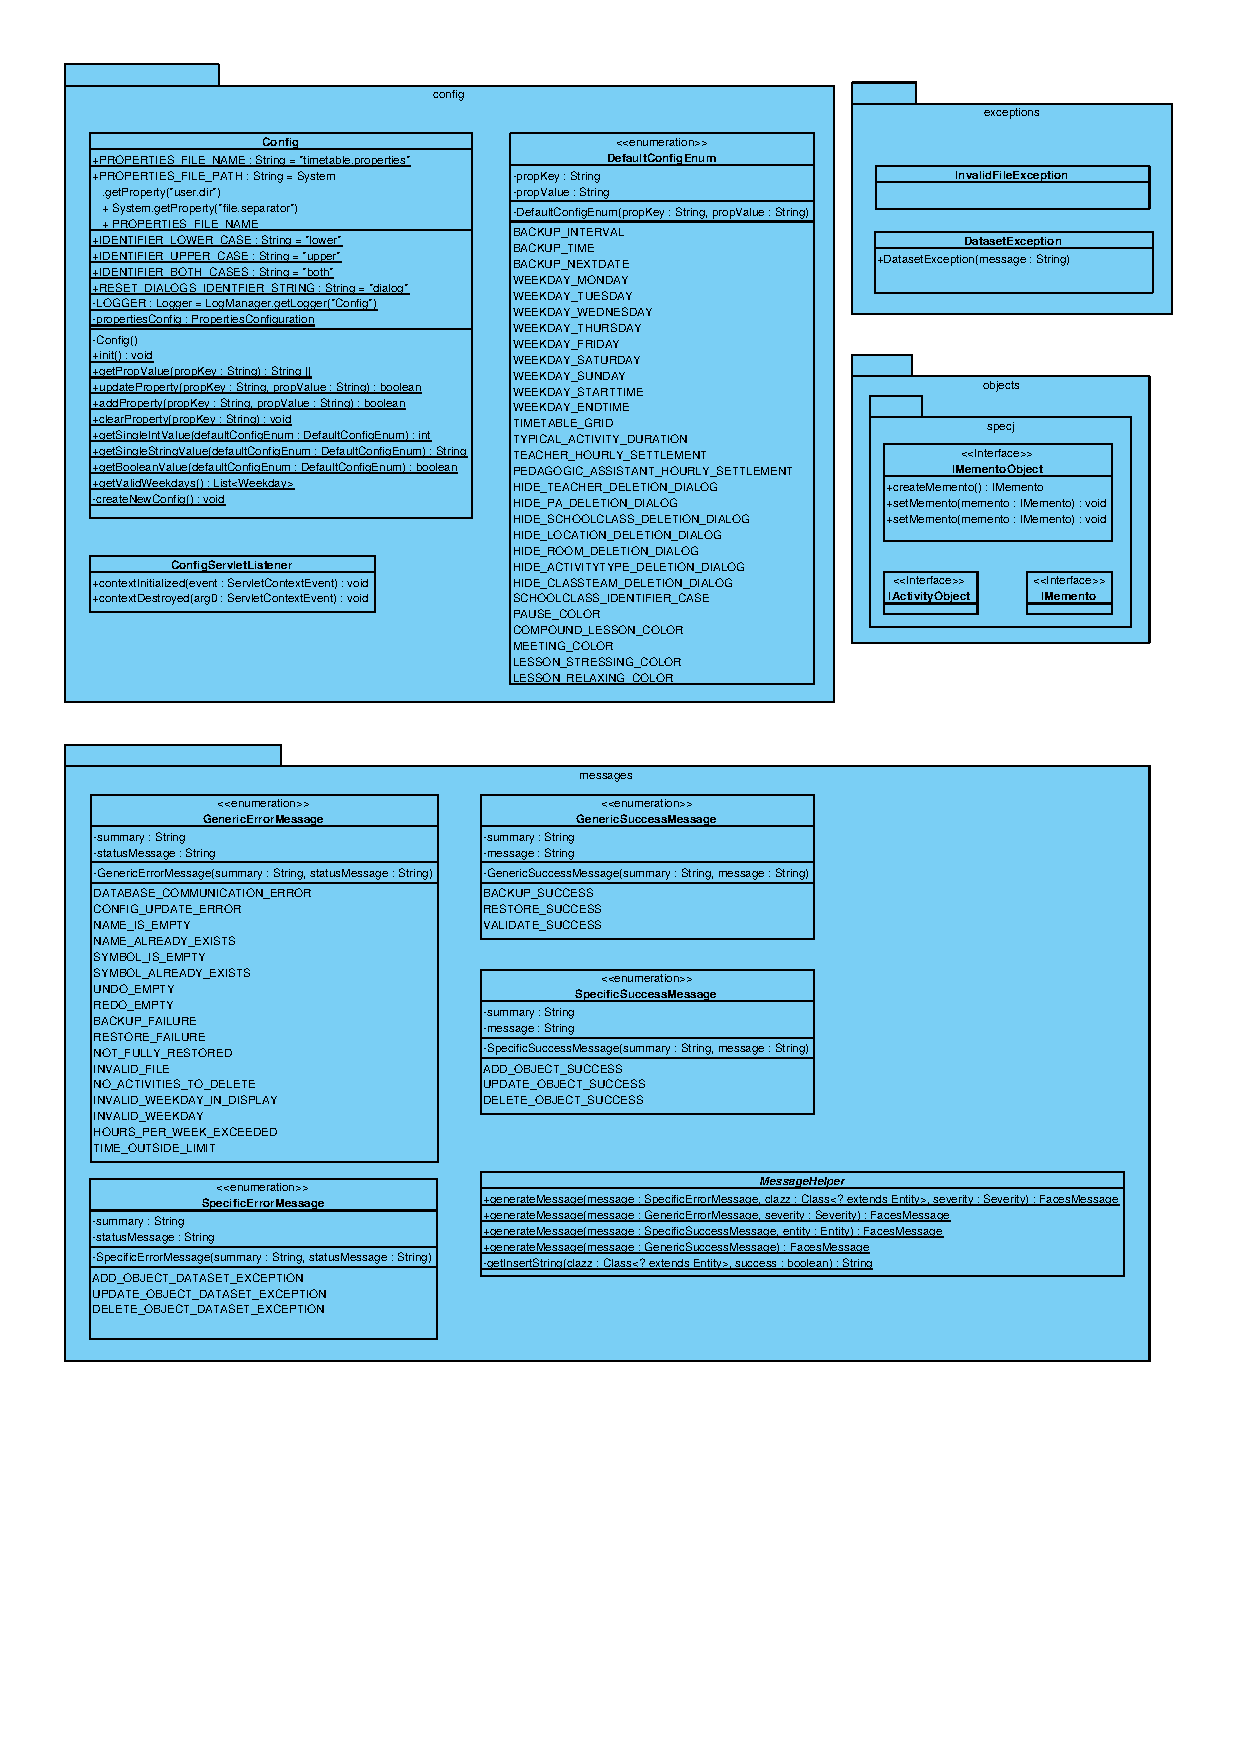
\includegraphics[width=\textwidth]{common.pdf}
\end{figure}
\newpage

\subsubsection{Objects}
\label{subsubsec:Objects}
%TODO: Beschreiben
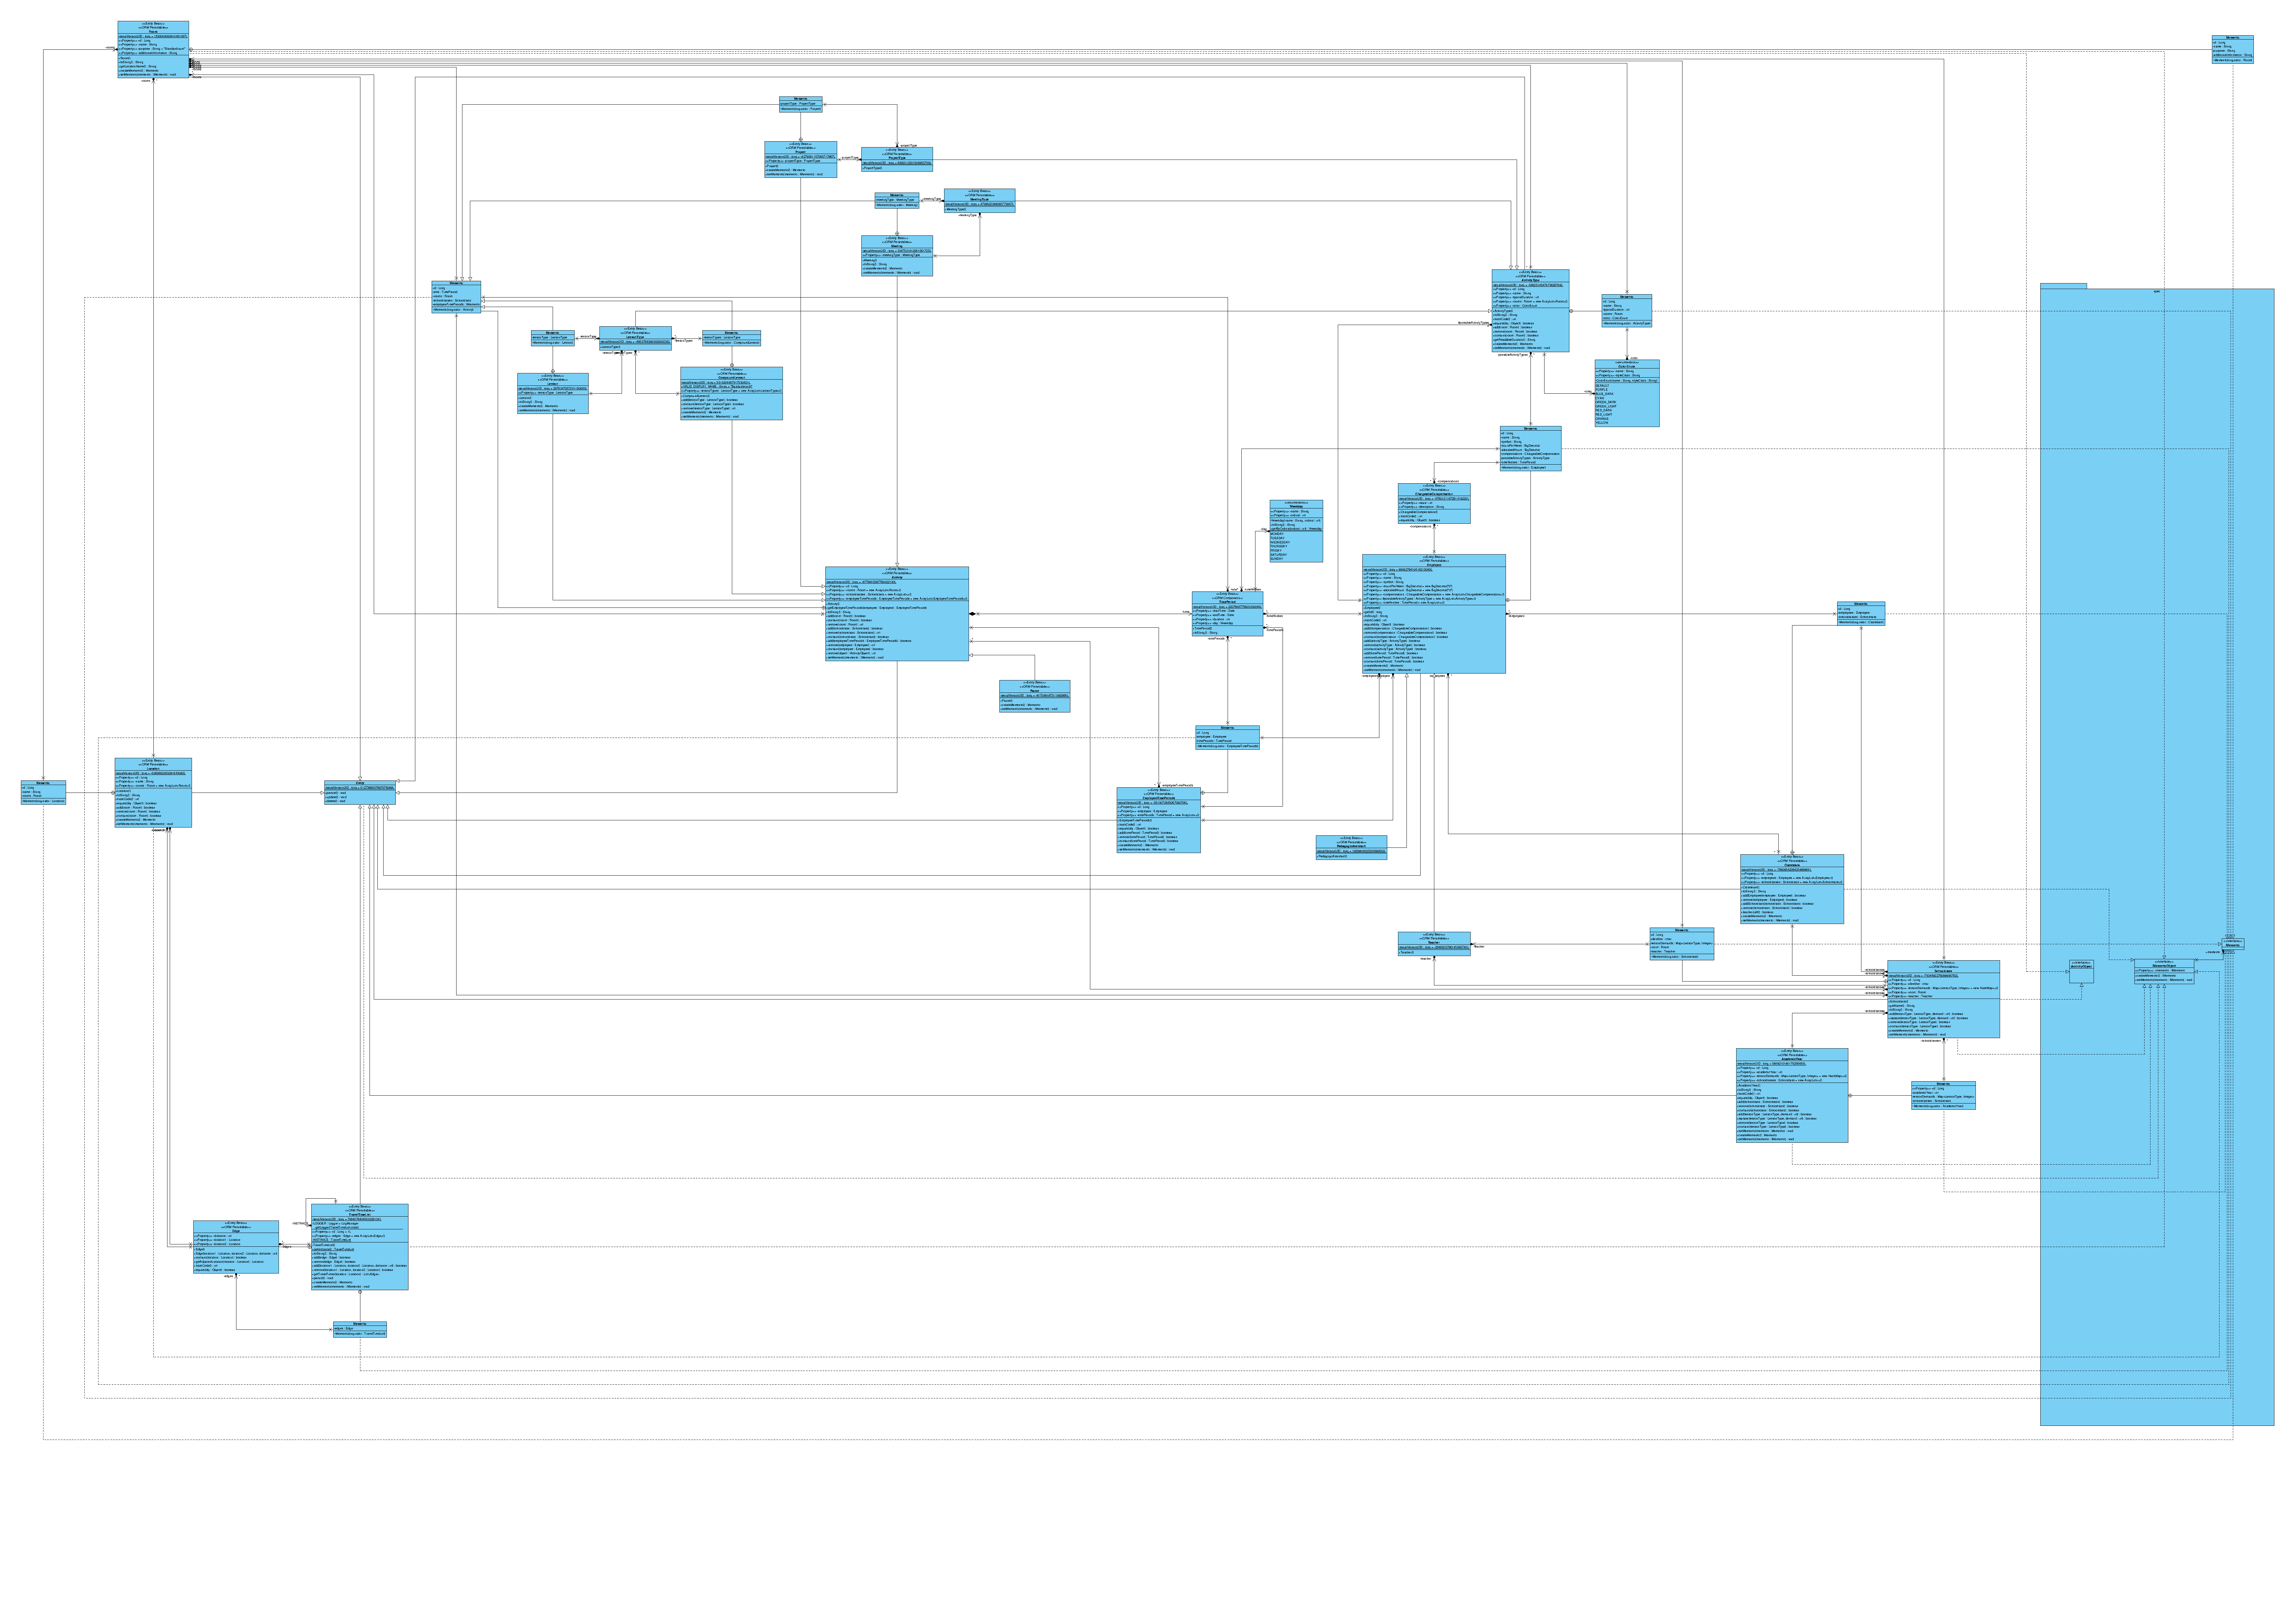
\includepdf[landscape]{objects.pdf}

\subsection{Logikschicht}
\label{sec:logic}
Auf der Logikebene wurde das Command-Pattern verwendet, um alle Undo und Redo für alle Aktionen anbieten zu können. Die entsprechenden Klassen befinden sich im Paket \textit{org.woym.logic.command}. \\
Das Interface \texttt{ICommand} spezifiziert die Methoden eines konkreten Commands. Implementiert wird das Interface von den Klassen \texttt{AddCommand}, \texttt{UpdateCommand}, \texttt{DeleteCommand} und \texttt{MacroCommand}.Für die Methoden gibt es eine klare Ausführungsreihenfolge. Nach Erzeugung eines ICommand-Objektes muss zunächst \textit{execute()} aufgerufen werden, danach dürfen alternierend \textit{undo()} und \textit{redo()} beliebig oft aufgerufen werden. \\
Neben den Commands befindet sich im Paket \textit{org.woym.logic.command} auch die Singleton-Klasse \texttt{CommandCreator}, welche als einzige öffentliche Methode die Methode \textit{createDeleteCommand(Entity)} anbietet. Diese erzeugt für ein übergebenes \textit{Entity}-Objekt ein MacroCommand zum Löschen dieses Objektes, welches in der korrekten Abfolge alle Abhängigkeiten auflöst, und gibt dieses zurück. Die Methode darf beliebig aufgerufen werden. Für nähere Informationen siehe JavaDoc.

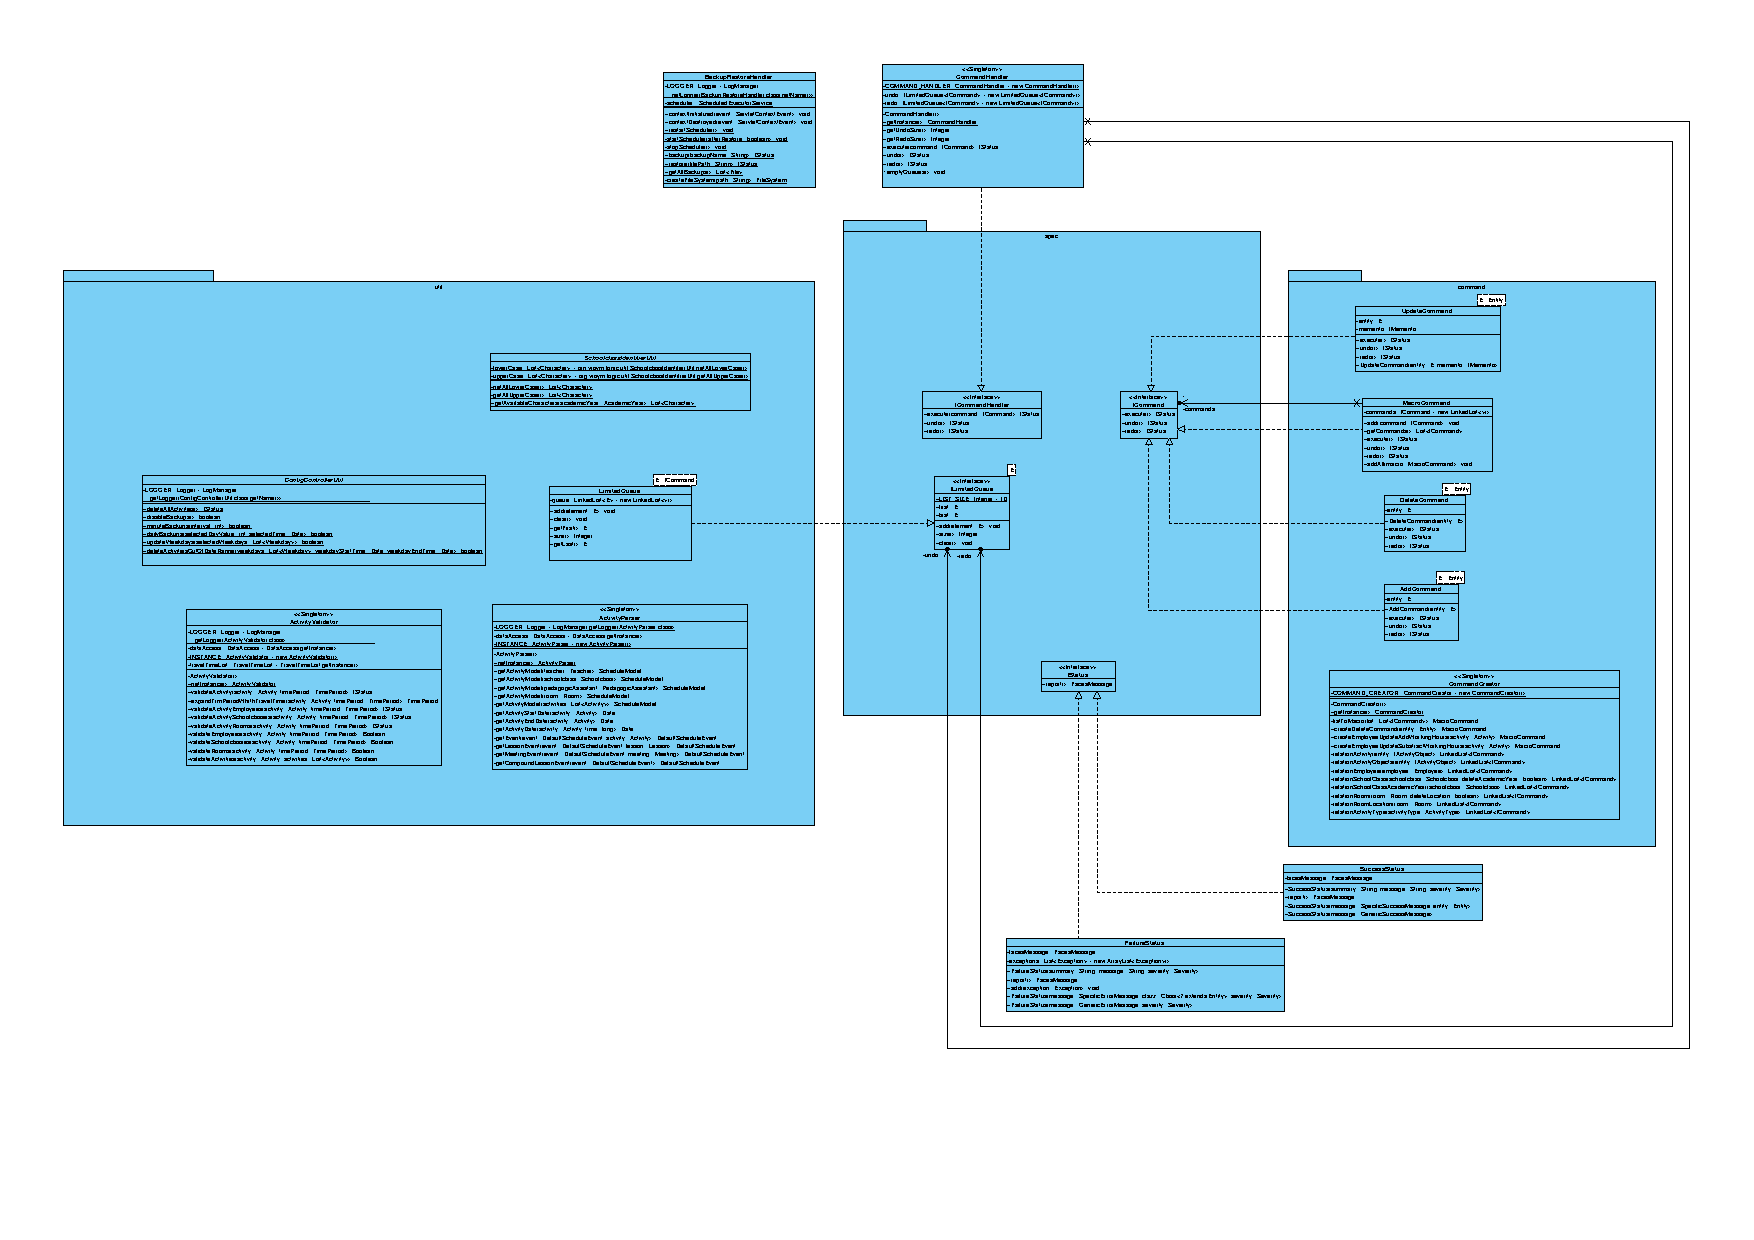
\includepdf[landscape]{logic.pdf}

\subsection{Persistenzschicht}
\label{sec:persistence}

%TODO: Beschreibung ggf. anpassen

Die Persistenzschicht ist für ein Single-User-System konzipiert und besteht aus drei Klassen. Die Singleton-Klasse \texttt{DataBase} stellt die unterste Ebene dar. Dort wird der EntityManager erzeugt, der für alle Datenbankanfragen von \texttt{DataAccess} verwendet wird. Außerdem bietet sie Methoden an, die ein Backup der Datenbank erzeugen bzw. ein Backup wiederherstellen. \texttt{DataBase} erweitert die Java-Klasse \texttt{Observable}, da es für die Wiederherstellung eines Backups notwendig ist, die Datenbank einmal komplett herunterzufahren und danach dementsprechend ein neuer EntityManager verwendet wird. Dies muss den beobachtenden Klassen mitgeteilt werden.\\
Die Singleton-Klasse \texttt{DataAccess} implementiert das Java-Interface \texttt{Observer} und wird bei Erzeugung bei \texttt{DataBase} als Observer registriert. Zudem implementiert sie das Interface \texttt{IDataAccess}, welches alle DAO-Interfaces implementiert und damit die notwendigen Datenzugriffsmethoden beschreibt. Die Klasse \texttt{DataAccess} stellt also für alle Klassen auf einer oberen Ebene die Schnittstelle zur Datenbank dar.\\
Die letzte Klasse der Persistenzschicht ist \texttt{DataBaseServletListener}, welche das Java-Interface \texttt{ServletContextListener} implementiert. Sie ruft mit dem Start des Servlet-Containers die \textit{setUp()}-Methode von \texttt{DataBase} auf.\\

Bevor die Methoden von \texttt{DataAcess} verwendet werden können, muss mindestens einmal die Methode \textit{setUp()} der Klasse \texttt{DataBase} aufgerufen werden, da diese den von \texttt{DataAccess} benötigten EntityManager erzeugt.\\
Die Methoden des Interfaces \texttt{IDataAccess} dürfen in beliebiger Reihenfolge aufgerufen werden. Methoden, welche als Rückgabewert eine Liste haben, geben in allen Fällen eine Liste zurück, diese kann also leer sein. Methoden, welche als Rückgabewert ein einzelnes Objekt einer Klasse besitzen, geben ein gemäß der JavaDoc-Beschreibung entsprechendes Objekt der Klasse oder \textbf{null} zurück, falls kein entsprechendes Objekt vorhanden ist. 


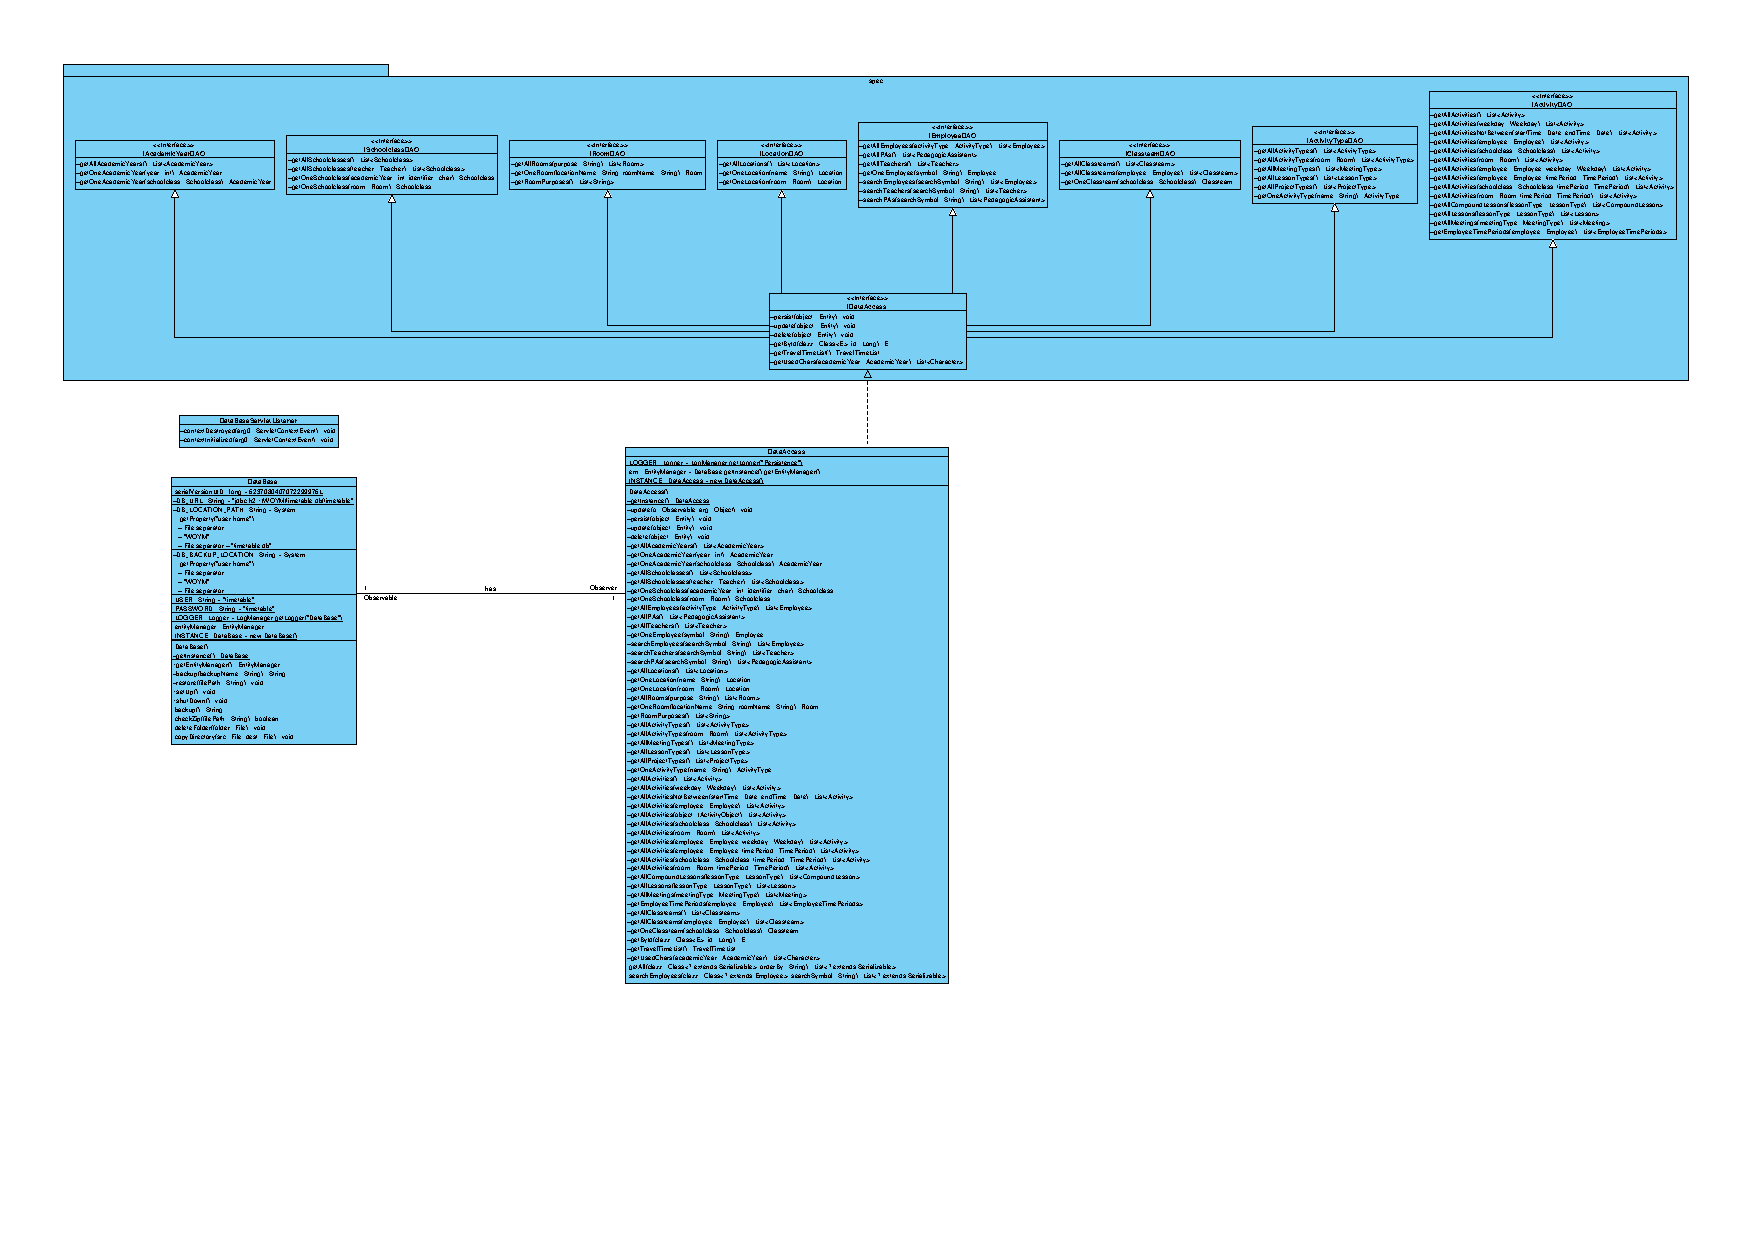
\includepdf[landscape]{persistence.pdf}


\section{Datensicht}
\label{sec:datensicht}
  
\subsection{Datenmodell}
Auf der folgenden Seite ist das Datenmodell dargestellt. Danach folgt eine Beschreibung der einzelnen Assoziationen.
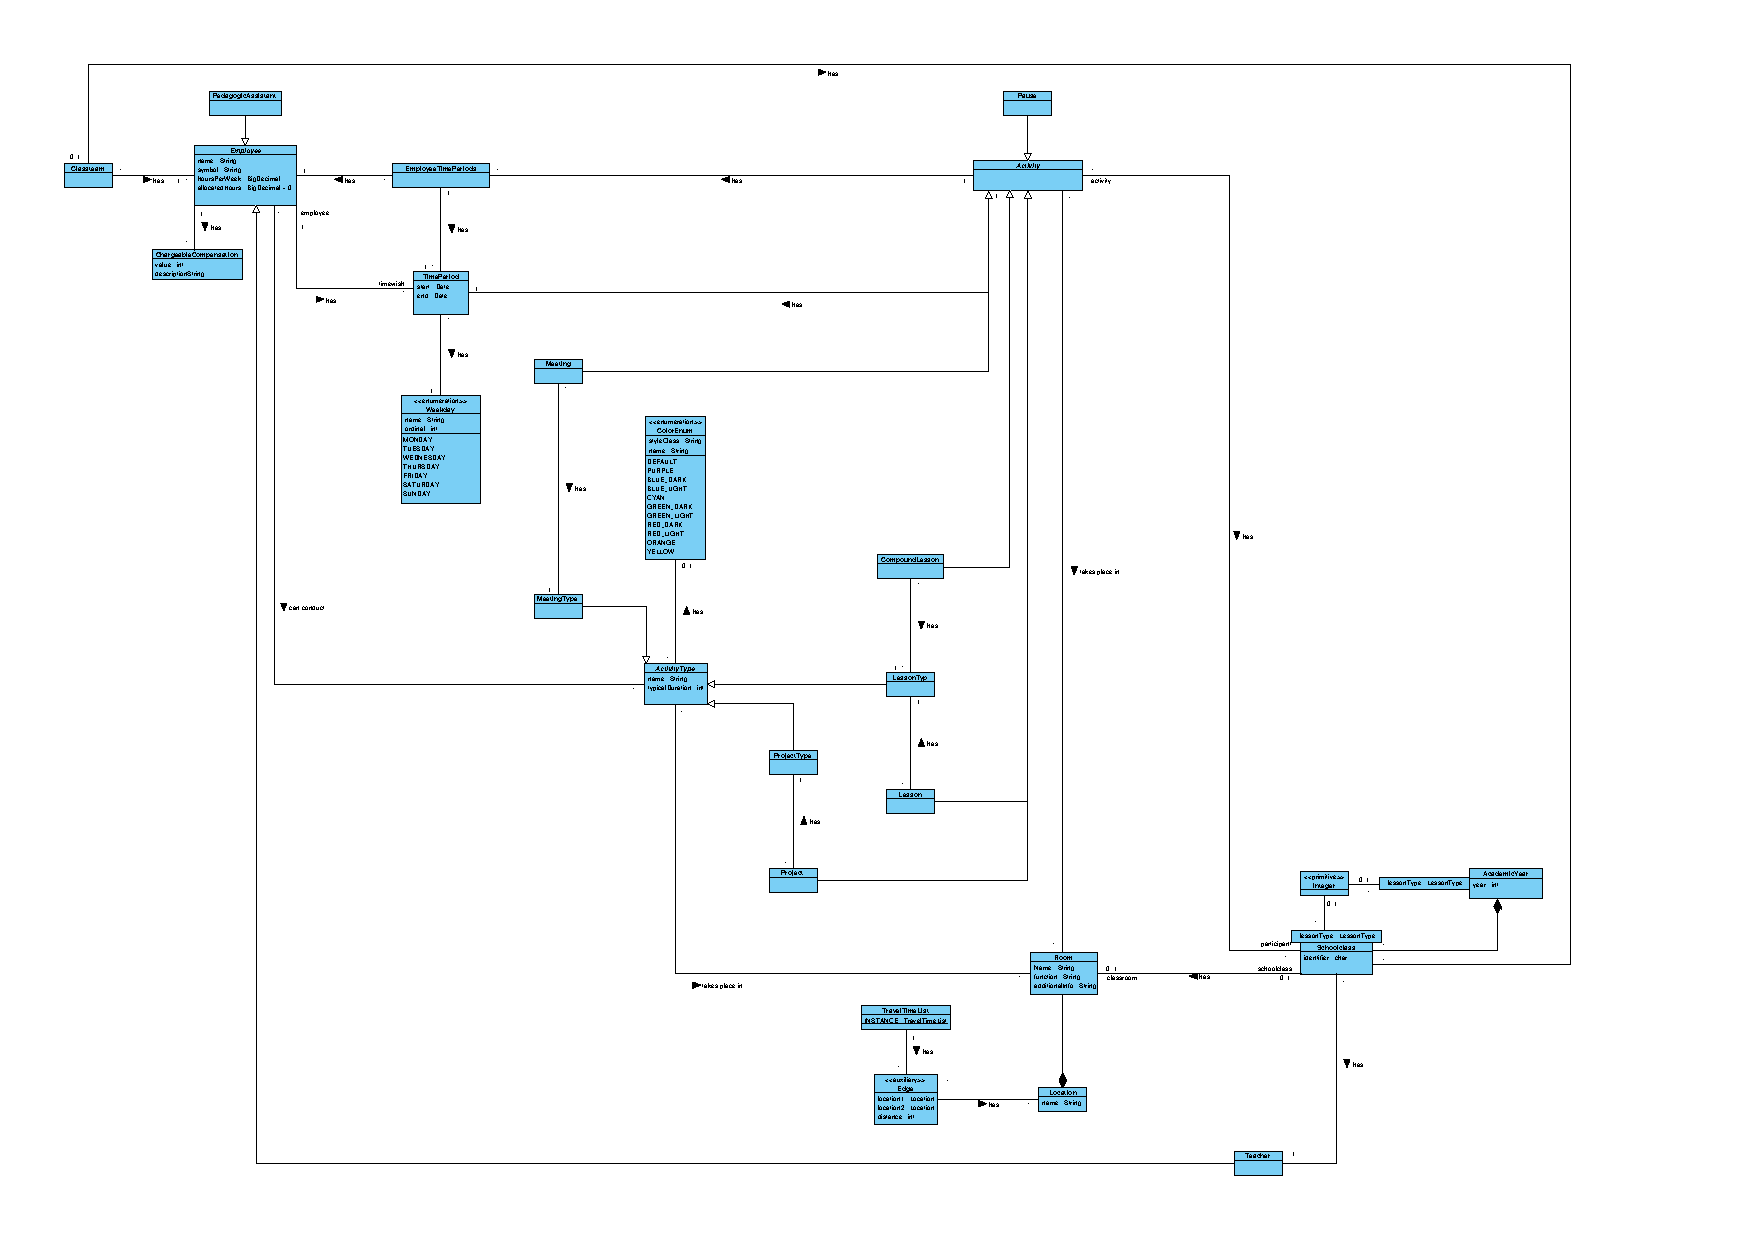
\includepdf[landscape]{datenmodell.pdf}
Im Folgenden soll die einzelnen Assoziationen erläutert werden.\\

\begin{tabularx}{\textwidth}{|p{0.6cm}|p{5cm}|X|}
\hline
\textbf{Nr.} & \textbf{Assoziation} & \textbf{Beschreibung} \\\hline
1 	& \textit{Employee} -- ChargeableCompensation	& Ein Mitarbeiter kann eine beliebige Anzahl
	an anrechenbaren Ersatzleistungen besitzen. Eine spezifische anrechenbare Ersatzleistung ist immer nur einem Mitarbeiter zugeordnet. \\\hline
2	& \textit{Employee} -- TimePeriod		& Ein Mitarbeiter hat eine beliebige Menge von 
	Zeiträumen als Zeitwünsche, also als Zeiten zu denen er gerne frei haben möchte. \\\hline
3	& \textit{Employee} -- \textit{ActivityType} & Einer beliebigen Anzahl von Mitarbeitern kann
	eine beliebige Anzahl von Aktivitätstypen als mögliche Stundeninhalte zugeordnet sein. Diese Assoziationen sind also komplett optional. \\\hline
4	& Schoolclass -- LessonType -- Integer \newline
	  AcademicYear -- LessonType -- Integer				& Eine Schulklasse und ein Jahrgang besitzen Unterrichtsbedarfe. Dies wird durch eine Zuordnung von Integer-Werten zu LessonType-Objekten realisiert. Jedes LessonType-Objekt darf in Kombination mit einer Klasse / einem Jahrgang nur einmal vorkommen. \\\hline
5	& Schoolclass -- Teacher 				& Eine beliebige Anzahl an Schulklassen hat genau
	einen Klassenlehrer. Ein Lehrer kann Klassenlehrer mehrere Schulklassen sein. \\\hline
6	& AcademicYear -- Schoolclass 			& Ein AcademicYear-Objekt besteht aus einer beliebigen 
	Anzahl Schoolclass-Objekten. Wird das AcademicYear-Objekt gelöscht, werden auch alle dazu gehörigen Schoolclass-Objekte gelöscht.\\\hline
7	& \textit{Activity} -- TimePeriod				& Einer Aktivität steht immer genau ein
	Zeitraum gegenüber.\\\hline
8	& \textit{Activity} -- Room						& Eine Aktivität ist mindestens einem, kann 
	aber mehreren Räumen zugeordnet sein.\\\hline
\end{tabularx}

\begin{tabularx}{\textwidth}{|p{0.6cm}|p{5cm}|X|}
\hline
9 	& \textit{Activity} -- EmployeeTimePeriods		& An einer Aktivität kann eine beliebige
	Anzahl an Mitarbeitern teilnehmen, da diese früher gehen oder später kommen können, wird jedem Mitarbeiter eine eigene Liste von Zeiträumen zugeordnet. Dies wird durch die Klasse \texttt{EmployeeTimePeriods} realisiert. Einer Aktivität kann eine beliebige Zahl von EmployeeTimePeriods-Objekten zugeordnet sein, aber ein spezifisches EmployeeTimePeriod-Objekt ist immer nur genau einer Aktivität zugeordnet. \\\hline
10	& \textit{Activity} -- Schoolclass				& Eine beliebige Anzahl von Aktivitäten
	besitzt eine beliebige Anzahl von Schulklassen als Teilnehmer. Schulklassen können die Aktivität nicht
	frühzeitig verlassen, daher gilt für sie der für die Aktivität festgelegte Zeitraum.\\\hline
11	& Meeting -- MeetingType 			 & Eine Aktivität vom Typ Meeting hat genau einen
	MeetingType. Ein MeetingType kann mehreren Aktivitäten vom Typ Meeting zugeordnet sein. \\\hline
12	& Project -- ProjectType			& Eine Aktivität vom Typ Project hat genau einen
	ProjectType. Ein ProjectType kann mehreren Aktivitäten vom Typ Project zugeordnet sein. \\\hline
13	& Lesson -- LessonType				& Eine Aktivität vom Typ Lesson hat genau einen
	LessonType. Ein LessonType kann mehreren Aktivitäten vom Typ Lesson zugeordnet sein. \\\hline
14	& CompoundLesson -- LessonType & Eine CompoundLesson (Bandunterricht) hat mindestens ein bis 
	beliebig viele LessonType-Objekte. \\\hline
15 	& EmployeeTimePeriods -- Employee 				& Eine beliebige Anzahl
	EmployeeTimePeriods-Objekte besitzt genau einen Lehrer. Ein Lehrer kann Teil einer beliebigen Anzahl von EmployeeTimePeriods-Objekten sein. \\\hline
16	& EmployeeTimePeriods -- TimePeriod 			& Ein EmployeeTimePeriods-Objekt besitzt
	mindestens eine bis beliebig viele TimePeriod-Objekte. Ein spezifisches TimePeriod-Objekt ist immer nur Teil von genau einem EmployeeTimePeriods-Objekt. \\\hline
\end{tabularx}

\begin{tabularx}{\textwidth}{|p{0.6cm}|p{5cm}|X|}
\hline
17 	& TimePeriod -- Weekday & Ein TimePeriod-Objekt hat genau einen Wochentag, ein Wochentag kann 
	mehreren TimePeriod-Objekten zugeordnet sein.\\\hline 
18	& Location -- Room						& Ein Standort besteht aus beliebig vielen Räumen. 
	Wird der Standort gelöscht, werden auch die Räume gelöscht.\\\hline
19	& \textit{ActivityType} -- Room					& Einer beliebigen Anzahl von Aktivitätstypen
	kann die Ausführung in einer beliebigen Anzahl von Räumen zugeordnet sein. \\\hline
20	& \textit{ActivityType} -- ColorEnum 		& Ein Aktivitätstyp hat genau eine Farbe oder keine 
	Farbe. Eine Farbe kann Teil mehrere Aktivitätstypen sein.\\\hline
21	& Classteam -- Schoolclass 					& Ein Klassenteam hat eine beliebige Anzahl 
	Schulklassen, eine Schulklasse ist aber immer nur genau einem oder keinem Klassteam zugeordnet.\\\hline
22	& Classteam -- Employee 					& Ein Klassteam hat mindestens einen bis zu 
	einer beliebigen Anzahl Mitarbeiter. Wobei Klassenteams ohne mindestens eine Lehrkraft auf Logikebene verhindert werden müssen. Ein Mitarbeiter kann Teil mehrere Klassenteams sein. \\\hline
23	& TravelTimeList -- Edge 					& Ein TravelTimeList-Objekt kann eine beliebige
	Anzahl von Edge-Objekten besitzen. Ein Edge-Objekt kann nur Teil eines TravelTimeList-Objektes sein. \\\hline
24	& Edge -- Location							& Einer beliebigen Anzahl von Edge-Objekten kann 
	eine beliebige Anzahl von Location-Objekten gegenüberstehen. Ein Edge-Objekt hat aber immer zwei disjunkte Location-Objekte.\\\hline 
\end{tabularx}
\subsection{Datentypen und Repräsentation von Multiplizitäten}

Diese Abbildung stellt eine andere Sichtweise auf das vorher gezeigte Klassendiagramm von. Es wurden alle Assoziationen weggelassen und dafür die Attribute an die entsprechenden Klassen eingetragen.
\begin{figure}[H]
\includegraphics[width=\textwidth]{datensicht.pdf}
\end{figure}


\subsection{Abbildung auf die Datenbank}
Die Abbildung auf die Datenbank erfolgt mithilfe des JPA-Frameworks Eclipselink. Damit muss lediglich darauf geachtet werden, die Attribute in den Klassen korrekt mit den One-To-Many- und Many-To-Many-Beziehungen gemäß des Datenmodells zu annotieren.


\section{Ausführungssicht}
\nurlangversion

\label{sec:ausfuehrung}

{\it
Die Ausführungssicht beschreibt das Laufzeitverhalten. Hier
werden die Laufzeitelemente aufgeführt und beschrieben, welche Module
sie zur Ausführung bringen. Ein Modul kann von mehreren
Laufzeitelementen zur Laufzeit verwendet werden. Die Ausführungssicht
beschreibt darüber hinaus, welche Laufzeitelemente spezifisch
miteinander kommunizieren. Zudem wird bei verteilten Systemen
(z.B. Client-Server-Systeme) dargestellt, welche Module von welchen
Prozessen auf welchen Rechnern ausgeführt werden.}


\section[Zusammenhänge zwischen Anwendungsfällen und Architektur]{Zusammenhänge zwischen Anwendungsfällen und Architektur\sectionmark{Zusammenhänge AF u. Architektur}}
\sectionmark{Zusammenhänge AF u. Architektur}
\label{sec:anwendungsfaelle}

{\it In diesem Abschnitt sollen Sequenzdiagramme mit Beschreibung(!)
  für \variante{zwei bis drei von Euch ausgewählte
    Anwendungsfälle}{einen von Euch ausgewählten Anwendungsfall}
  erstellt werden. Ein Sequenzdiagramm beschreibt den
  Nachrichtenverkehr zwischen allen Modulen, die an der Realisierung
  des Anwendungsfalles beteiligt sind.  \variante{Wählt die
    Anwendungsfälle so, dass nach Möglichkeit alle Module Eures
    entworfenen Systems in mindestens einem Sequenzdiagramm
    vorkommen. Falls Euch das nicht gelingt, versucht möglichst viele
    und die wichtigsten Module abzudecken.}{Dazu könnt ihr Euch einen
    Anwendungsfall heraussuchen, der möglichst viele Module der
    Architektur abdeckt. In SWP-2 werden wir mehrere Anwendungsfälle
    betrachten und eine umfangreichere Abdeckung der Architektur
    anstreben.} }

\section{Evolution}
\nurlangversion

\label{sec:evolution}

{\it
  Beschreibt in diesem Abschnitt, welche Änderungen Ihr
  vornehmen müsst, wenn sich Anforderungen oder Rahmenbedingungen
  ändern. Insbesondere sollten hierbei die in der
  Anforderungsspezifikation unter "`Ausblick"' bereits genannten
  Punkte behandelt werden.}

\dots


\end{document} 
